%\documentclass[13pt,letterpaper]{llncs2e/llncs}
\documentclass[11pt,letterpaper]{article}

%\usepackage{amsfonts}
\usepackage[margin=1in]{geometry}

\usepackage{booktabs}
\usepackage[capitalise]{cleveref}
%\usepackage{hyperref}
\usepackage{color}
\usepackage[dvipsnames]{xcolor}

\usepackage[group-separator={\,}]{siunitx}
\usepackage[noend]{algorithm2e}
\DontPrintSemicolon

\usepackage[sort,numbers]{natbib}
\renewcommand{\bibnumfmt}[1]{#1.}
%\bibliographystyle{IEEEtranN}
\usepackage{pgfplots}
%\usetikzlibrary{matrix}
%\usepgfplotslibrary{groupplots}
%\pgfplotsset{compat=newest}

%opening
\title{FgClust, a fast and scalable algorithm for generating high-quality clusters of biological sequences}
\author{XiaoFei Zhao, ShingHei Zhan}

\begin{document}

\maketitle

\begin{abstract}
Clustering of biological sequences is a fundamental problem.
We developed FgClust, a novel multi-threaded sequence-clustering algorithm.
FgClust uses a variant of greedy set cover instead of greedy incremental update, uses min-hash values instead of short words, and uses the length of non-centroid query sequence minus infix Levenshtein distance instead of sequence identity.
We compared FgClust with Linclust, MMSeqs2, CD-HIT, and kClust
%, and kClust 
on PDB, UniRef, and Pfam.
We compared FgClust with VSEARCH and CD-HIT-EST on Rfam.
Compared with the aforementioned state-of-the-arts algorithms.
FgClust always achieves faster runtime and better trade-off between sensitivity and specificity, except that Linclust is approximately 4 times faster but also generates up to 100\% more clusters than FgClust.
Similar to Linclust, the observed runtime of FgClust scales linearly with respect to input size.
\end{abstract}

\section{Introduction}

Sequence clustering is a fundamental problem in Biology.
Clustering of nucleic or amino acid sequences lowers the redundancy in sequence databases.
In addition, sequences in the same cluster can be assumed to have similar biological properties.
%Clustering of short reads produced by sequencers can detect and correct sequencing error.
We developed FgClust, a novel sequence-clustering algorithm that can scale to hundreds of millions of sequences.
FgClust generates better-quality clusters and is faster than all known published sequence-clustering algorithms, except that FgClust is slower than Linclust by a constant multiplicative factor.
However, Linclust generates up to 100\% more clusters than FgClust.
%FgClust has the potential to generate better taxonomy.

%\section{Related works}

%Clustering of biological sequences has a long history.
%\Citet{holm1998removing} observed that two sufficiently long protein sequences that share no common decapeptide must have at most 90\% sequence identity.
%Based on this observation, \citet{holm1998removing} developed a method called nrdb90 that clusters protein sequences at 90\% sequence identity.
%However, nrdb90 is slow and cannot run with sequence identity of less than 90\%.
%\Citet{li2001clustering} observed that two protein sequences of lengths \(L_1\) and \(L_2\) must share at least \(x\) peptides, or equivalently short words, of length \(y\) in order to share at least \(z\)\% sequence identity, 
%	where \(L_1\), \(L_2\), \(x\), \(y\), and \(z\) are mathematically interdependent variables.
%\Citet{li2001clustering} therefore generalized the decapeptide filter into short-word filter.
%Based on this observation, \citet{li2001clustering} developed a method called CD-HI that clusters protein sequences at 70\% or more sequence identity.
%\Citet{li2001clustering} introduced the notion of greedy al update, where sequences are longest-first sorted and each sequence either belongs to an already formed cluster or forms a new cluster. 
%Since then, nearly all clustering methods used greedy incremental update, so we will assume such unless explicitly stated otherwise.
%CD-HI is both significantly faster and can cluster at lower sequence identity than nrdb90 without significantly sacrificing neither sensitivity nor specificity.
%However, the exponential increase in the size of a typical protein database made CD-HI too slow to be practical.
%\Citet{li2002tolerating} extended the work of \citet{li2001clustering} by filtering out sequence pairs that are likely to share less than a certain sequence-identity cutoff.
%\Citet{li2002tolerating} observed that two protein sequences of lengths \(L_1\) and \(L_2\) are not necessarily , but likely, to share at least \(x\) peptides of length \(y\) in order to share at least \(z\)\% sequence identity.
%Based on this extension, \citet{li2002tolerating} developed a method called CD-HIT that clusters protein sequences at 50\% or more sequence identity. 
%At the same sequence-identity cutoff, CD-HIT produces 0.4\% more clusters than but is about 100 times faster than CD-HI.
%\Citet{li2006cd} observed that the algorithm in CD-HIT can be further extended to cluster nucleotide sequences and to compare two biological databases.
%\Citet{fu2012cd} used OpenMP to parallelize CD-HIT.

%\Citet{edgar2010search} developed a method called USEARCH which performs database search by sequence identity. 
%In addition of using the short-word filter used by CD-HIT, USEARCH only searches a fixed maximum number of top hit target sequences per query sequence.  
%\Citet{edgar2010search} also developed UCLUST which clusters biological sequences using the distance computed by USEARCH.
%USEARCH and UCLUST are both closed-source commercial programs, so \citet{rognes2016vsearch} developed VSEARCH which is open-source and similar to USEARCH and UCLUST in terms of functionality and performance.

%Clustering of short reads produced by Next-Generation Sequencing (NGS) is also an ongoing research topic.
%\Citet{zorita2015starcode} developed starcode, an algorithm for clustering sequences at high global similarity cutoff based edit distance.
%Starcode is especially useful for detection and correction of sequencing errors. 

\section{Approach}

\begin{algorithm}
\SetKwInOut{Parameter}{Parameter}
	\KwIn{Randomly shuffled nucleotide or amino-acid sequences}
	\KwOut{Clustering of input sequences, where each cluster has one representative}
	\Parameter{Percent edit-similarity \textnormal{percsim} which affects any variable with the symbol \(x\)}
	\caption{FgClust}
	\label{alg.mainLoop}
	\SetKwFunction{proc}{can-cover}
	\SetKwProg{myproc}{Subroutine}{}{}
	\myproc{\proc\((s_1, s_2):\)}{
		Compute the number \(d\) of single-character edits to make \(s_2\) a substring of \(s_1\).\;
		\KwRet \(4/5 \le \text{length}(s_1)/\text{length}(s_2) \le 5/4\)
		and \((s_2-d) \ge \sqrt{25^2 + (s_2 \times \textnormal{percsim})^2}\).\; 
	}
	Apply Murphy10 alphabet reduction on input if input is protein sequences.\;
%	\If{input is protein sequences}{
%		Reduce amino-acid alphabet for computation of long words, minhash values, and edit-similarities.\;
%	}
	\For{each sequence in input}{
		Index some equally spaced long words, in the form of hash values, in the sequence.\;
	}
	\For{each indexed long word, in parallel}{
		\If{the long word occurs more than 1000 times in the index}{
			Uniformly and independently sample 800 pairs of sequences sharing this long word.\;
			%For each pair, compute the minhash values shared between the two sequences in the pair.\;
			Pick 10 pairs with the highest number of minhash values shared by the pair.\;
			Initialize the number of true hits to zero.\;
			\For{each pair \((s_1, s_2)\) in these 10 pairs}{
				\lIf{\proc\((s_1, s_2)\)}{
					Increment the number of true hits by one.%.\;
				}
			}
			\If{the number of true hits is less than 5}{
				Remove the long word, which is regarded as non-informative, from the index.\;
			}
		}
%		\If{the long word is abundant and sequences sharing this long word are usually not similar}{
%			Remove the long word, which is regarded as non-informative, from the index.
%		}
	}
	\For{each sequence in input, in parallel}{
		Let the sequence be represented by its 32 minhash values.\;	
	}
	Divide input sequences into chunks of sequences.\;
	\For{each chunk}{
		\For{each sequence \(s_1\) in the chunk, in parallel \textnormal{(LOOP2)}}{
			\If{\(s_1\) is covered less than \(x\) times where \(x\in[4,6]\)}{
				Let \(S_2\) be the list of sequences sharing at least one long word with \(s_1\).\;
				Sort \(S_2\), in descending order, by the number of minhash values shared with \(s_1\).\;
				%Remove \(S_2\)  that shares less than certain number of minhash values with \(s_1\).\;
				Initialize \(n\) to \(x\), where \(x\in[20,60]\).\;
				\For{each sequence \(s_2\) in \(S_2\) such that \(s_1\) and \(s_2\) share enough minhash values}{
					\If{\(s_2\) is covered less than \(x\) times where \(x\in[13,21]\)}{
						\uIf{\proc\((s_1, s_2)\)}{
							Will apply the following update after LOOP2: let \(s_1\) cover \(s_2\).\;
							Increase \(n\) by \(x\) such that \(n\) is capped at \(x+10\), where \(x\in[20,60]\).\;
						}\uElse{
							Decrease \(n\) by one.\;
						}
					}
					\lIf{\(n\) is zero}{
						exit loop.%.\;
					}
				}
			}
		}
		%\(\mathbb{C}=\mathbb{C} \bigcup C\).\;
	}
	Perform greedy set-cover on input sequences to produce a set \(R\) of representatives.\;
	For each input sequence, find its best representative in \(R\);
	\newline
%	, where elements covered by a set are stored in \texttt{std::vector}.
%	\For{Each sequence in input}{
%		Let the sequence be covered by the representative produced by the set-cover to minimize the edit-similarity from the input sequence to the representative.
%	}
\end{algorithm}

\Citet{li2001clustering} introduced the notion of greedy incremental update.
Greedy incremental update iterates through each sequence, usually in descending order of sequence length, and each iterated sequence either forms a new cluster or is assigned to an existing cluster.
Thus, any not-yet-iterated sequence that can be assigned to an already iterated sequence cannot be a centroid.
However, a not-yet-iterated sequence can be a better centroid than the already iterated sequence.
Thus, such premature determination of centroid can result in more clusters of worse quality.
Instead, FgClust delays the determination of centroid and performs lookahead. 
More specifically, only a not-yet-iterated sequence that can be assigned to sufficient number of already iterated sequences cannot be a centroid.
Then, FgClust makes clustering decisions using an algorithm that is less greedy than the greedy incremental update.
This reduction in greediness induces less number of clusters with better centroids and thus increases sensitivity and specificity.
We implemented a linear-time and memory-efficient version of the greedy set-cover algorithm,
	where each representative sequence represents and covers its member sequences.

\subsection{Improved sequence search}

\Citet{li2002tolerating} used short-word filter in CD-HIT.
Short-word filter estimates the similarity between two sequences by counting their common short words.
Short word is also known as short k-mer.
However, a typical biological sequence has hundreds of short words.
Instead, we transform short words into hash values and select a fixed number of lowest hash values.
Then, we use the lowest hash values, or equivalently min-hash values, as short words.
This reduction in short words reduces runtime.
We implemented a version of rolling hash that produces pseudo-random hash values.

Sequence identity is the number of matches divided by the length of the shorter sequence in an alignment.
Usually, the blosum62 matrix with an affine gap penalty is used to compute such alignment.
However, such computation of alignment is time-consuming.
Moreover, sequence identity ignores deletions in the longer sequence.
Thus, sequence identity can overestimate the relatedness between two sequences.
Sequence alignment maximizes alignment score instead of the number of matches.
Thus, the biological relatedness implied by number of matches can be lower than the biological relatedness implied by alignment score.
Thus, sequence identity can underestimate the relatedness between two sequences.
%Conservation of biological function requires smaller number of matches of conserved residues than matches of non-conserved residues. 
%However, smaller number of matches decreases sequence identity.
%Unfortunately, substitution matrices such as blosum62 tend to produce matches of conserved residues.
%Thus, sequence identity computed with a substitution matrix can underestimate the true biological similarity.
Instead of using sequence identity, we used edit-similarity.
The edit-similarity between a query and a target is defined as follows: 
	the length of the target minus the minimum number of single-character edits required such that the edited target is a substring of the query, divided by the length of the target.
%Then, edit-similarity is used as sequence identity.
Edit-similarity takes less time to compute than sequence identity \citep{vsovsic2017edlib}.
Moreover, edit-similarity is more correlated with biological relatedness than sequence identity, as shown in \cref{table:pdb,fig:pfam,fig:rfam}.
Therefore, the use of edit-similarity instead of sequence identity improves sensitivity, specificity, and runtime.
We used the library implemented by \citet{vsovsic2017edlib} to compute edit-similarity.

In addition of developing the previously mentioned novel sequence-search techniques, we developed some variants of traditional sequence-search techniques.
Given a query sequence, FgClust searches only each database sequence that shares at least one informative long word with the query sequence.
A long word is a k-mer and is represented by its hash value.
FgClust ignores uninformative and abundant long words to improve runtime.
A long word is uninformative if and only if two uniformly, randomly, and independently sampled sequences that share this long word usually do not share sufficiently high edit-similarity.
Therefore, two sequences sharing only uninformative and abundant long words will be ignored in sequence search.
Two or more amino acids with similar biochemical properties can be reduced into one amino acid.
%For example, the unreduced alphabet of 20 standard amino acids can be reduced into an alphabet of 10-19 amino acids.
FgClust uses the Murphy10 amino-acid alphabet reduction suggested by \citet{murphy2000simplified} to improve sensitivity.
FgClust computes long words, min-hash values, and edit-similarities all with the reduced alphabet.
%If the edit-similarity threshold is between 81\% and 100\%, then the alphabet is not reduced. 
%If the edit-similarity threshold is between 62\% and 80\%, then the alphabet is reduced into 15 amino acids.
%If the edit-similarity threshold is less than 62\%, then the alphabet is reduced into 10 amino acids. 
FgClust sorts in descending order target candidates by the number of min-hash values shared between the query and each target candidate.
FgClust initializes and then keeps track of a number of remaining attempts.
Each true-positive  target candidate increases the number of remaining attempts.
Each false-positive target candidate decreases the number of remaining attempts.
The number of remaining attempts is capped and thus cannot exceed certain value.
The search prematurely terminates when the number of remaining attempts reaches zero, similar to the pruning strategy used by \citet{edgar2010search}.
%FgClust uses OpenMP to perform sequence search on multiple queries in parallel \citep{dagum1998openmp}.

\section{Evaluation on biological databases}

We evaluated every state-of-the-arts clustering algorithm on every gold-standard biological database.
Only the memory-limited 32-bit version of UCLUST is free and UCLUST is not open source \citep{edgar2010search}.
Thus, we omitted UCLUST in our evaluation.
Before any evaluation, we shuffled, by using a random-number generator with the same seed, the sequences in each biological database.
Thus, our evaluation results were both deterministically and yet pseudo-randomly generated to be both reproducible and yet unaffected by the order of sequences in a database.
Thus, every researcher can reproduce our evaluation results.
All evaluations are done on a ``CentOS release 6.6'' server that runs on an ``Intel(R) Xeon(R) CPU E5-2660 0 @ 2.20GHz'' CPU with 32 threads.

\subsection{Evaluation on protein databases}

We compared FgClust with CD-HIT version 4.6 \citep{fu2012cd}, Linclust commit 91644c75 \citep{steinegger2017linclust}, MMSeqs commit 91644c75 \citep{steinegger2017mmseqs2}, and kClust version 1.0 \citep{hauser2013kclust}. kClust always has the worst sensitivity-specificity trade-off and is too time-consuming to be practical (data not shown). Therefore, the results of evaluation on kClust are not shown.

\begin{table}%[!htbp]
	\centering
	\caption{
		The sequences of all monomeric proteins in PDB accessed in January 1st 2017 are given as input to each program \citep{berman2006protein}. 
		Each program is run with each intra-cluster similarity threshold to generate each set of clusters.
		For each set of clusters, the number of clusters characterized by intra-cluster template-modeling (TM) scores inclusively below each threshold is tabulated.
		The intra-cluster TM score of a cluster is the lowest TM score between the representative sequence in the cluster as template and each represented sequence in the cluster.
		A cluster with an intra-cluster TM-score of at most 0.5 contains at least one outlier in terms of three-dimensional structure and is thus of bad quality.
		FgClust produces the least number of bad-quality clusters.
		The runtime of each program is too short to measure wall-clock time and scalability.
	}
	\begin{tabular}{l c c c c c c c c c c}
		
		\toprule
		Program & intra-cluster & \multicolumn{9}{c}{intra-cluster TM scores} \\
		& similarity & 
		  \(\le\) 0.2 & \(\le\) 0.3 & \(\le\) 0.4 & \(\le\) 0.5 
		& \(\le\) 0.6 & \(\le\) 0.7 & \(\le\) 0.8 & \(\le\) 0.9 & \(\le\) 1.0 \\
		\midrule
		
		FgClust  & 50 & 7 & 45 & 137 & 283 & 510 & 875 & 1399 & 2205 & 16520 \\
		FgClust  & 70 & 7 & 42 & 131 & 252 & 443 & 759 & 1226 & 1954 & 17940 \\
		FgClust  & 90 & 7 & 35 & 111 & 219 & 380 & 633 & 1021 & 1719 & 19327 \\

		Linclust & 50 & 29 & 118 & 253 & 402 & 657 & 1030 & 1566 & 2362 & 16964 \\
		Linclust & 70 & 30 & 119 & 245 & 378 & 612 & 957 & 1445 & 2181 & 17765 \\
		Linclust & 90 & 23 & 89 & 187 & 316 & 502 & 796 & 1219 & 1917 & 19220 \\
	
		MMseqs2  & 50 & 30 & 125 & 264 & 416 & 695 & 1109 & 1647 & 2477 & 15159 \\
		MMseqs2  & 70 & 30 & 116 & 250 & 380 & 617 & 981 & 1464 & 2201 & 17160 \\
		MMseqs2  & 90 & 35 & 113 & 222 & 357 & 557 & 835 & 1263 & 1958 & 18782 \\
		
		%kClust    & 90 & 8 & 355 & 4358 & 5274 & 5365 & 5397 & 5425 & 5463 & 5513 & 19713 \\
		
		CD-HIT   & 50 & 40 & 138 & 280 & 440 & 694 & 1104 & 1627 & 2437 & 15657 \\
		CD-HIT   & 70 & 39 & 126 & 247 & 379 & 584 & 912 & 1388 & 2113 & 17603 \\
		CD-HIT   & 90 & 29 & 114 & 223 & 342 & 513 & 771 & 1158 & 1846 & 19119 \\
		

		%kClust    & 70 & 15 & 383 & 4469 & 5435 & 5523 & 5557 & 5584 & 5620 & 5662 & 17681 \\
		

		%kClust    & 50 & 15 & 402 & 4477 & 5428 & 5515 & 5548 & 5574 & 5607 & 5644 & 16111 \\
		
%		FgClust  & 50 & 0 & 7 & 46 & 137 & 283 & 510 & 877 & 1403 & 2214 & 16575 \\
%		Linclust & 50 & 0 & 29 & 118 & 253 & 402 & 656 & 1032 & 1565 & 2368 & 16964 \\
%		CD-HIT   & 50 & 0 & 40 & 138 & 280 & 438 & 694 & 1107 & 1631 & 2445 & 15712 \\
%		
%		FgClust  & 70 & 0 & 7 & 42 & 131 & 253 & 444 & 761 & 1228 & 1960 & 18010 \\
%		Linclust & 70 & 0 & 30 & 119 & 245 & 378 & 614 & 957 & 1446 & 2190 & 17828 \\
%		CD-HIT   & 70 & 0 & 39 & 126 & 247 & 380 & 585 & 913 & 1390 & 2118 & 17668 \\
%		
%		FgClust  & 90 & 0 & 7 & 35 & 111 & 219 & 380 & 633 & 1022 & 1724 & 19400 \\
%		Linclust & 90 & 0 & 23 & 89 & 188 & 316 & 502 & 796 & 1221 & 1922 & 19298 \\
%		CD-HIT   & 90 & 0 & 29 & 114 & 223 & 342 & 514 & 772 & 1160 & 1852 & 19194 \\
%		
		\bottomrule
	\end{tabular}
	\label{table:pdb}
\end{table}
We assessed the specificity of FgClust using experimentally verified data.
We downloaded all monomeric proteins with experimentally determined structures deposited into PDB before January 2nd 2017 \citep{berman2006protein}.
The sequence of each protein is extracted.
If an extracted sequence has at least 11 non-ambiguous amino acids and at least 90\% amino acids of the extracted sequence are non-ambiguous, then the extracted sequence is kept.
From these kept sequences, every sequence-clustering algorithm produces a set of clusters.
Within each cluster, the template-modeling (TM) score between the representative sequence and each represented sequence is computed by TM-Align developed by \citet{zhang2005tm}.
The lowest such TM score within each cluster is extracted and referred to as intra-cluster TM score.
The number of such intra-cluster TM scores below each TM score threshold are shown in \cref{table:pdb}.
The lower such extracted TM scores are, the less specific the clustering algorithm is.
\Cref{table:pdb} shows that FgClust produces the fewest number of clusters with low intra-cluster TM scores.
Usually, two proteins are in the same fold if and only if these two proteins share a TM-score of at least 0.5 \citep{xu2010significant}, where a protein fold is defined by the arrangement of the secondary structure elements relative to each other in space.
\Cref{table:pdb} shows that other algorithms produce about 50\% more clusters with intra-cluster TM scores of less than 0.5 than FgClust.
Therefore, FgClust is significantly more specific than other algorithms in terms of experimentally observed protein structures.

\begin{figure}%[!htbp]
	\centering
	\begin{tabular}{c c}
		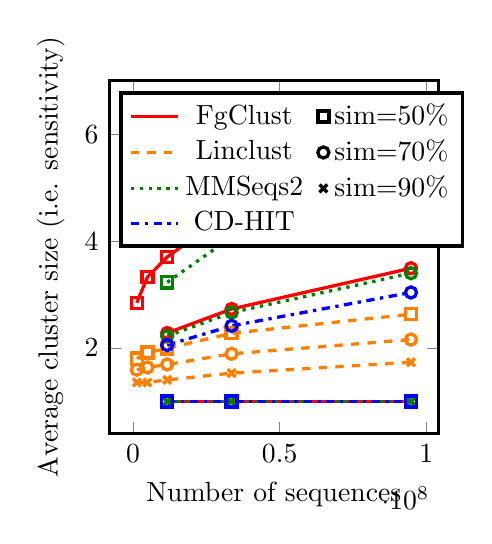
\begin{tikzpicture}
		%\draw[->,very thick](4,0.5)--(4,4)node
		%[midway,below,sloped]{more sensitive};
		\begin{axis}[very thick,
		width=0.475\textwidth,height=0.5\textwidth,
		mark options={solid},
		%xmode=log,
		%ymode=log,
		ymax=7,%xmax=1.1e8,
		xlabel=Number of sequences,
		ylabel={Average cluster size (i.e. sensitivity)},
		legend columns=4,
		transpose legend,
		legend entries={FgClust~~,
			Linclust~~,
			MMSeqs2~~,
			CD-HIT~~,
			sim=50\%,sim=70\%,sim=90\%},
		legend pos=north west]
		\addlegendimage{,red}
		\addlegendimage{dashed,orange}
		\addlegendimage{dotted,Green}
		\addlegendimage{dash dot,blue}
		\addlegendimage{only marks,mark=square}
		\addlegendimage{only marks,mark=o}
		\addlegendimage{only marks,mark=x}
		
		\addplot[color=red,mark=square] coordinates {
			(1306318,  1306318 / 458904)
			(4910948,  4910948 / 1475783)
			(11659891, 11659891 / 3150744)
			(33613081, 33613081 / 7317301)
			(94756963, 94756963 / 15652579)
		}; %FgClust 50
		\addplot[color=red,mark=o] coordinates {
			(11659891, 11659891 / 5111980)
			(33613081, 33613081 / 12311744)
			(94756963, 94756963 / 27135041)
		}; %FgClust 70
		\addplot[color=red,mark=x] coordinates {
			(11659891, 11659891 / 11659891)
			(33613081, 33613081 / 33613081)
			(94756963, 94756963 / 94756963)
		}; %FgClust 90
		
		\addplot[dashed,color=orange,mark=square] coordinates {
			(1306318,  1306318 / 725566)
			(4910948,  4910948 / 2562086)
			(11659891, 11659891 / 5847706)
			(33613081, 33613081 / 14766033)
			(94756963, 94756963 / 35983786)
		}; %Linclust 50
		\addplot[dashed,color=orange,mark=o] coordinates {
			(1306318,  1306318 / 819293)
			(4910948,  4910948 / 3000298)
			(11659891, 11659891 / 6889416)
			(33613081, 33613081 / 17768118)
			(94756963, 94756963 / 43908412)
		}; %Linclust 70
		\addplot[dashed,color=orange,mark=x] coordinates {
			(1306318,  1306318 / 962908)
			(4910948,  4910948 / 3625681)
			(11659891, 11659891 / 8306445)
			(33613081, 33613081 / 21974288)
			(94756963, 94756963 / 54672623)
		};
		
		\addplot[dotted,color=Green,mark=square] coordinates {
			(11659891, 11659891 / 3611747)
			(33613081, 33613081 / 8247473)
			(94756963, 94756963 / 17764174)
		}; % mmseqs2 50
		\addplot[dotted,color=Green,mark=o] coordinates {
			(11659891, 11659891 / 5244520)
			(33613081, 33613081 / 12622595)
			(94756963, 94756963 / 27872093)
		};
		\addplot[dotted,color=Green,mark=x] coordinates {
			(11659891, 11659891 / 11659891)
			(33613081, 33613081 / 33613081)
			(94756963, 94756963 / 94756963)
		};
		
		\addplot[dash dot,color=blue,mark=square] coordinates {
			(11659891, 11659891 / 11659891)
			(33613081, 33613081 / 33613081)
			(94756963, 94756963 / 94756963)
		};
		\addplot[dash dot,color=blue,mark=o] coordinates {
			(11659891, 11659891 / 5671408)
			(33613081, 33613081 / 13921644)
			(94756963, 94756963 / 31180026)
		};
		\addplot[dash dot,color=blue,mark=square] coordinates {
			(11659891, 11659891 / 11659891)
			(33613081, 33613081 / 33613081)
			(94756963, 94756963 / 94756963)
		};
		\end{axis}
		\end{tikzpicture}
		&
		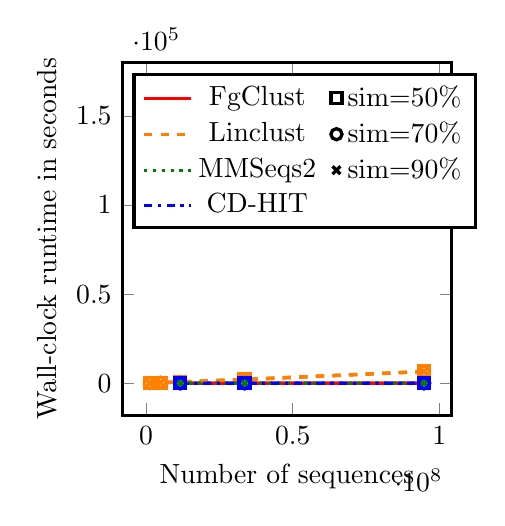
\begin{tikzpicture}
		\begin{axis}[very thick,
		width=0.475\textwidth,height=0.5\textwidth,
		mark options={solid},
		%xmode=log,
		%ymode=log,
		ymax=3600*50,%xmax=1.1e8,
		xlabel=Number of sequences,
		ylabel=Wall-clock runtime in seconds,
		legend columns=4,
		transpose legend, 
		legend entries={FgClust~~,
			Linclust~~,
			MMSeqs2~~,
			CD-HIT~~,
			sim=50\%,sim=70\%,sim=90\%},
		legend pos=north west]
		\addlegendimage{,red}
		\addlegendimage{dashed,orange}
		\addlegendimage{dotted,Green}
		\addlegendimage{dash dot,blue}
		\addlegendimage{only marks,mark=square}
		\addlegendimage{only marks,mark=o}
		\addlegendimage{only marks,mark=x}
		
		\addplot[color=red,mark=square] coordinates {
			(11659891, 11659891 / 3150744)
			(33613081, 33613081 / 7317301)
			(94756963, 94756963 / 15652579)
		};
		\addplot[color=red,mark=o] coordinates {
			(11659891, 11659891 / 5111980)
			(33613081, 33613081 / 12311744)
			(94756963, 94756963 / 94756963)
		};
		\addplot[color=red,mark=x] coordinates {
			(11659891, 11659891 / 11659891)
			(33613081, 33613081 / 33613081)
			(94756963, 94756963 / 94756963)
		};
		\addplot[dashed,color=orange,mark=square] coordinates {
			(1306318,  63.14)
			(4910948,  276.93)
			(11659891, 645.21)
			(33613081, 2015.70)
			(94756963, 6476.00)
		}; %linclust 50
		\addplot[dashed,color=orange,mark=o] coordinates {
			(1306318,  68.50)
			(4910948,  304.54)
			(11659891, 698.67)
			(33613081, 2110.71)
			(94756963, 6580.54)
		};
		\addplot[dashed,color=orange,mark=x] coordinates {
			(1306318,  72.65)
			(4910948,  310.12)
			(11659891, 699.81)
			(33613081, 2186.68)
			(94756963, 6575.24)
		};
		
		\addplot[dotted,color=Green,mark=square] coordinates {
			(11659891, 11659891 / 3611747)
			(33613081, 33613081 / 8247473)
			(94756963, 94756963 / 17764174)
		};
		\addplot[dotted,color=Green,mark=o] coordinates {
			(11659891, 11659891 / 6889416)
			(33613081, 33613081 / 17768118)
			(94756963, 94756963 / 94756963)
		};
		\addplot[dotted,color=Green,mark=x] coordinates {
			(11659891, 11659891 / 11659891)
			(33613081, 33613081 / 33613081)
			(94756963, 94756963 / 94756963)
		};
		
		\addplot[dash dot,color=blue,mark=square] coordinates {
			(11659891, 11659891 / 11659891)
			(33613081, 33613081 / 33613081)
			(94756963, 94756963 / 94756963)
		};
		\addplot[dash dot,color=blue,mark=o] coordinates {
			(11659891, 11659891 / 5671408)
			(33613081, 33613081 / 33613081)
			(94756963, 94756963 / 94756963)
		};
		\addplot[dash dot,color=blue,mark=square] coordinates {
			(11659891, 11659891 / 11659891)
			(33613081, 33613081 / 33613081)
			(94756963, 94756963 / 94756963)
		};
		\end{axis}
		\end{tikzpicture}
		
		
	\end{tabular}
	\caption{
		UniRef100-2.0, UniRef100-12.0,
		UniRef100-2011-01, UniRef100-2014-01, and UniRef100-2017-01 
		are five releases of the UniRef100 database and capture the growth of UniRef100 from July 2004 to January 2017 \citep{suzek2007uniref}. %are available at \texttt{ftp://ftp.uniprot.org/pub/databases/uniprot/previous\_releases/}.
		These five releases have \SI{1306318}, \SI{4910948}, \SI{11659891}, \SI{33613081}, and \SI{94756963} sequences, respectively \citep{suzek2007uniref}.
		We ran each program on each UniRef100 release with each intra-cluster similarity threshold to generate each set of clusters.
		Cluster quality is not assessed due to the lack of ground truth.
		\label{fig:uniref}
	}
\end{figure}

%\begin{table}%[!htbp]
%	\centering
%	\caption{	
%		All sequences in a specified version of UniRef are given as input to each program \citep{suzek2007uniref}. 
%		Each program is run with each intra-cluster similarity threshold to generate each set of clusters.
%		Runtime is measured in seconds. % TODO!!!: update data
%		Cluster quality is not assessed due to lack of ground truth.
%	}
%	\begin{tabular}{l c c c c c c c}
%		\toprule
%		Program & intra-cluster & \multicolumn{2}{c}{UniRef100-2011-01}
%		& \multicolumn{2}{c}{UniRef100-2014-01}
%		& \multicolumn{2}{c}{UniRef100-2017-01} \\ 
%		& similarity    & cluster count & runtime
%		& cluster count & runtime
%		& cluster count & runtime \\
%		
%		\midrule
%		FgClust  & 90 & \SI{7539905} & 43 & \SI{19864156} & 117 & \SI{48113438} & 442 \\
%		Linclust & 90 & \SI{8079020} & 11 & \SI{21434130} & 35  & \SI{53391467} & 109 \\
%		CD-HIT   & 90 & \SI{7627325} & 46 & \SI{20173024} & 132 & \SI{49200220} & 724 \\
%		
%		FgClust  & 70 & \SI{5531553} & 36 & \SI{13482152} & 127 & \SI{29938650} & 563 \\
%		Linclust & 70 & \SI{6192036} & 11 & \SI{15548951} & 33  & \SI{37011492} & 104 \\
%		CD-HIT   & 70 & \SI{5671370} & 41 & \SI{13921545} & 110 & \SI{31178816} & 525 \\
%		FgClust  & 50 & \SI{3911258} & 62 & \SI{8991582}  & 276 & \SI{19288061} & 1443 \\
%		Linclust & 50 & \SI{5114737} & 10 & \SI{12535362} & 30  & \SI{29461562}  & 92 \\
%		CD-HIT   & 50 & timeout & \(>\)5000 & timeout & \(>\)5000 & timeout & \(>\)5000 \\
%		\bottomrule
%	\end{tabular}
%	\label{fig:uniref}
%\end{table}

We assessed the sensitivity and runtime of FgClust.
We downloaded the three releases of UniRef100 \citep{suzek2007uniref} shown in \cref{fig:uniref}.
Unlike NR, all previous releases of UniRef100 are available for download.
Unlike UniProtKB, the number of protein sequences in UniRef100 as a function of release date is monotonically increasing.
Therefore, we used UniRef100 instead of NR and UniProtKB in this assessment.
From each release of UniRef, we extracted protein sequences.
From these extracted sequences, each sequence-clustering algorithm produces a set of clusters.
The number of clusters produced by each algorithm and the runtime of each algorithm are shown in \cref{fig:uniref}.
A more sensitive clustering algorithm produces less number of clusters with larger average cluster size.
\Cref{fig:uniref} shows that FgClust produces the least number of clusters with the largest average cluster size.
Therefore, FgClust is the most sensitive.
Moreover, \cref{fig:uniref} shows that FgClust is always faster than CD-HIT and MMSeqs2.
FgClust is slower but significantly more sensitive than Linclust.
In fact, Linclust produces more than 100\% more clusters than FgClust at 50\% intra-cluster similarity.
CD-HIT always times out at 50\% intra-cluster similarity.
%Therefore, only FgClust is useful in practice at 50\% intra-cluster similarity.

\begin{figure}%[!htbp]
	\centering
		\begin{tabular}{c c}
			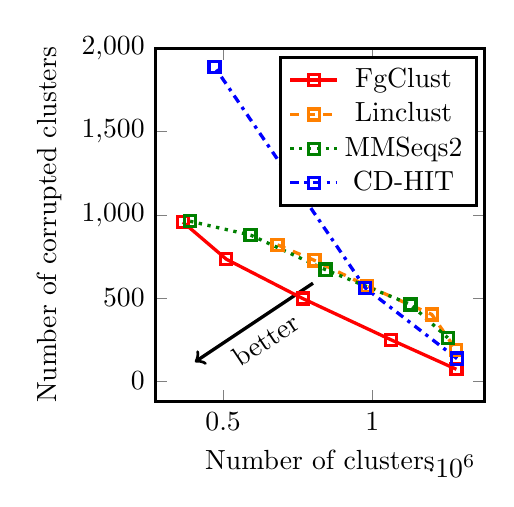
\begin{tikzpicture}
			\draw[->,very thick](2,1.5)--(0.5,0.5)node
			[midway,below,sloped]{better};
			\begin{axis}[very thick,
			mark options={solid},
			width=0.475\textwidth,
			height=0.5\textwidth,
			%ymode=log,
			ymax=2000,
			xlabel=Number of clusters,
			ylabel=Number of corrupted clusters]
%			\addplot[color=red,mark=square] coordinates {
%				(1285018, 111)
%				(983569, 430)
%				(595103, 777)
%			};
			\addplot[color=red,mark=square] coordinates {
				(1282321, 71)
				(1063439, 248)
				(767432, 496)
				(510593, 733)
				(365198, 956)
				%(595103, 777)
			};
			\addlegendentry{FgClust}
			\addplot[dashed,color=orange,mark=square] coordinates {	
				(682422, 819)
				(806160, 726)
				(982978, 572)
				(1199664, 401)
				(1281061, 188)
			};
			\addlegendentry{Linclust}
			\addplot[dotted,color=Green,mark=square] coordinates {
%				(1253466, 260)
%				(843812,  671)
%				(389818,  961)
				(389251,  961)
				(592123,  878)
				(843097,  670)
				(1128425, 461)
				(1253416, 260)
			};
			\addlegendentry{MMSeqs2}
%			\addplot[color=cyan,mark=square] coordinates {
%				(1283109, 1578)
%				(947926, 123004)
%				(504755, 153861)
%			};
%			\addlegendentry{kClust}
			\addplot[dash dot,color=blue,mark=square] coordinates {
				(1284610, 135)
				(976699, 560)
				(471363, 1889)
			};
			\addlegendentry{CD-HIT}

			\end{axis}
			\end{tikzpicture}
			&
			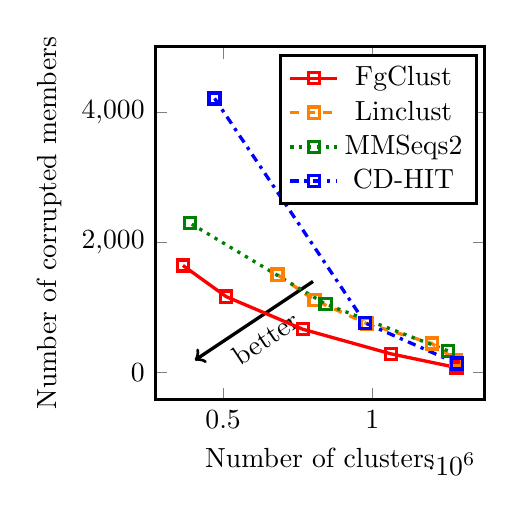
\begin{tikzpicture}
			\draw[->,very thick](2,1.5)--(0.5,0.5)node
			[midway,below,sloped]{better};
			
			\begin{axis}[very thick,
			mark options={solid},
			width=0.475\textwidth,
			height=0.5\textwidth,
			%ymode=log,
			ymax=5000,
			xlabel=Number of clusters,
			ylabel=Number of corrupted members]
			\addplot[color=red,mark=square] coordinates {
				(1282321, 76)
				(1063439, 285)
				(767432, 663)
				(510593, 1163)
				(365198, 1642)
%				(1285018, 114)
%				(983569, 506)
%				(595103, 1229)
			};
			\addlegendentry{FgClust}
			\addplot[dashed,color=orange,mark=square] coordinates {	
				(682422, 1501)
				(806160, 1111)
				(982978, 749)
				(1199664, 445)
				(1281061, 193)
			};
			\addlegendentry{Linclust}
			\addplot[dotted,color=Green,mark=square] coordinates {
				(1253466, 333)
				(843812,  1049)
				(389818,  2290)
			};
			\addlegendentry{MMSeqs2}
			\addplot[dash dot,color=blue,mark=square] coordinates {
				(1284610, 139)
				(976699, 759)
				(471363, 4207)
			};
			\addlegendentry{CD-HIT}

			\end{axis}
			\end{tikzpicture}
		\end{tabular}
	\caption{Results of clustering Pfam-A.seed release 31.0 \citep{finn2016pfam}.
		On each line, the five marks from top left to bottom right correspond to the five sequence-similarity cutoffs of 50\%, 60\%, 70\%, 80\%, and 90\%, respectively.
		A cluster is corrupted if and only if at least one member in the cluster is corrupted.
		A cluster member is corrupted if and only if the member belongs to a Pfam family that the representative of the cluster does not belong to.
		The runtime of each program is too short to measure wall-clock time and scalability.
		\label{fig:pfam}
	}
%	\begin{tabular}{l c c c c}
%		\toprule
%		Program & intra-cluster & 
%		\multicolumn{3}{c}{statistics for evaluation on Pfam-A.seed} \\
%		& similarity    & cluster & corrupted cluster & corrupted member \\
%		\midrule
%		FgClust  & 90 & 1285018 & 111 & 114 \\
%		Linclust & 90 & 1281035 & 189 & 198 \\
%		CD-HIT   & 90 & 1284610 & 135 & 139 \\
%		
%		FgClust     & 70 & 983161 & 429 & 506 \\
%		Linclust & 70 & 971547 & 585 & 706 \\
%		CD-HIT   & 70 & 976699 & 560 & 759 \\
%		
%		FgClust     & 50 & 592585 & 776 & 1206 \\
%		Linclust & 50 & 664691 & 835 & 1450 \\
%		CD-HIT   & 50 & 471363 & 1889 & 4207 \\
%		
%		\bottomrule
%	\end{tabular}
	
\end{figure}
We assessed the sensitivity and specificity of FgClust using manually curated data.
We downloaded the manually curated seed A dataset from Pfam version 31.0 \citep{finn2016pfam}.
We ran each clustering algorithm on this dataset.
A corrupted cluster contains at least two sequences that belong to two different Pfam families.
A corrupted cluster member belongs to a Pfam family that the representative of this cluster does not belong to.
A more sensitive clustering algorithm produces fewer clusters.
A more specific clustering algorithm produces fewer corrupted clusters and fewer corrupted cluster members.
\Cref{fig:pfam} shows that FgClust generates much less number of corrupted clusters and cluster members given the same number of clusters generated.
Therefore, FgClust achieves the best sensitivity-specificity trade-off.
CD-HIT has the worst sensitivity-specificity trade-off at low sequence identity presumably because inferring biological relatedness from low sequence identity is highly error-prone.
Linclust and MMSeqs2 use e-value in addition of sequence identity and therefore do not suffer from such drop in sensitive-specificity trade-off.
Linclust and MMSeqs2 can merge clusters.
An false-positive merging step corrupts only one cluster but can corrupt multiple cluster members.
Therefore, Linclust and MMSeqs2 generate high numbers of corrupted cluster members compared with the numbers of corrupted clusters.


\subsection{Evaluation on nucleotide databases}

\begin{figure}%[!htbp]
	\centering
\begin{tabular}{c c}
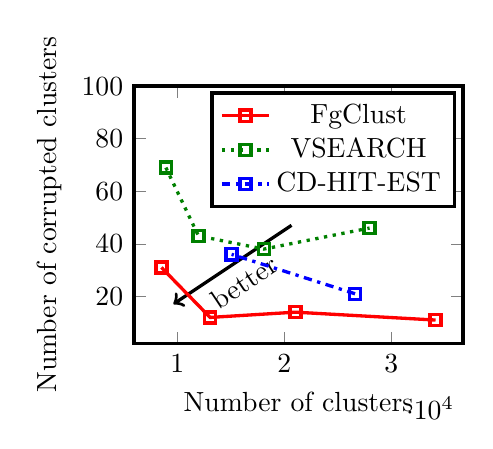
\begin{tikzpicture}
\draw[->,very thick](2,1.5)--(0.5,0.5)node
[midway,below,sloped]{better};
\begin{axis}[very thick,
mark options={solid},
width=0.475\textwidth,
height=0.4\textwidth,
ymax=100,%ymode=log,
xlabel=Number of clusters,
ylabel=Number of corrupted clusters]
\addplot[color=red,mark=square] coordinates {
	%(7675, 135)
	(8514, 31)
	(13062, 12)
	(21032, 14)
	(34130, 11)
};
\addlegendentry{FgClust}
\addplot[dotted,color=Green,mark=square] coordinates {
	%(7509, 126)
	(8929, 69)
	(11978, 43)
	(18085, 38)
	(27963, 46)
};
\addlegendentry{VSEARCH}
\addplot[dash dot,color=blue,mark=square] coordinates {
	(26608, 21)
	(15074, 36)
};
\addlegendentry{CD-HIT-EST}
\end{axis}
\end{tikzpicture}
&
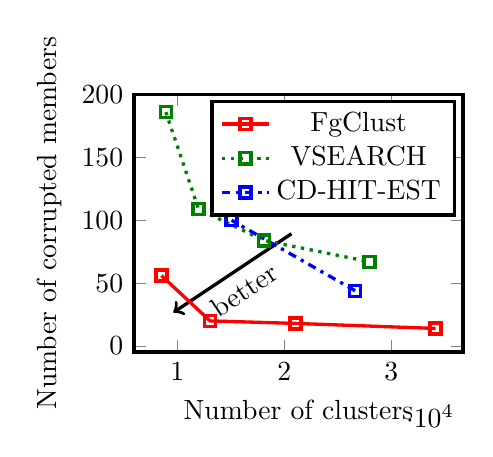
\begin{tikzpicture}
\draw[->,very thick](2,1.5)--(0.5,0.5)node
[midway,below,sloped]{better};
\begin{axis}[very thick,
mark options={solid},
width=0.475\textwidth,
height=0.4\textwidth,
ymax=200,%ymode=log,
xlabel=Number of clusters,
ylabel=Number of corrupted members]
\addplot[color=red,mark=square] coordinates {
	%(7675, 341)
	(8514, 56)
	(13062, 20)
	(21032, 18)
	(34130, 14)
};
\addlegendentry{FgClust}
\addplot[dotted,color=Green,mark=square] coordinates {
	%(7509, 1958)
	(8929, 186)
	(11978, 109)
	(18085, 84)
	(27963, 67)
};
\addlegendentry{VSEARCH}
\addplot[dash dot,color=blue,mark=square] coordinates {
	(26608, 44)
	(15074, 100)
};
\addlegendentry{CD-HIT-EST}
\end{axis}
\end{tikzpicture}
\end{tabular}
\caption{Results of clustering Rfam.seed release 12.3 \citep{nawrocki2014rfam}.
	On each line, the four marks from left to right correspond to the four sequence-similarity cutoffs of 60\%, 70\%, 80\%, and 90\%, respectively. CD-HIT-EST does not run with any sequence-similarity cutoff of less than 80\%.
	A cluster is corrupted if and only if at least one member in the cluster is corrupted.
	A cluster member is corrupted if and only if the member belongs to an Rfam family that the representative of the cluster does not belong to.
	The runtime of each program is too short to measure wall-clock time and scalability.
	\label{fig:rfam}
}
\end{figure}
We assessed the sensitivity and specificity of FgClust using manually curated nucleotide data. 
We downloaded the seed dataset from Rfam version 12.3 \citep{nawrocki2014rfam}.
We ran FgClust, VSEARCH \citep{rognes2016vsearch}, and CD-HIT-EST \citep{fu2012cd} on this dataset.
Evaluation criteria on Rfam and Pfam are similar.
\Cref{fig:rfam} shows that FgClust produces about 50\% less clusters given the same number of corrupted clusters and about 60\% less corrupted clusters given the same number of clusters.
Therefore, FgClust is significantly more sensitive at the same specificity and significantly more specific at the same sensitivity.
Therefore, FgClust performs the best for the Rfam dataset.

\section{Conclusion}

%Clustering of biological sequences is a fundamental problem.
We developed FgClust, a novel algorithm for clustering biological sequences.
FgClust is in general more sensitive, more specific, and faster than known published clustering algorithms.
We observed that greedy incremental update may not select the optimal centroid during each incremental update.
Therefore, FgClust detects sufficient number of sequence pairs such that, in each pair, the first can represent the second.
Then, FgClust uses greedy set cover to cluster all sequences based on such pairing.
We observed that there are too many short words in a protein sequence.
Therefore, FgClust uses min-hash values instead of short words.
We observed that sequence identity is not sufficiently correlated with biological relatedness and requires the time-consuming computation of alignment.
Therefore, FgClust uses edit-similarity instead of sequence identity.
%Edit-similarity is defined as one minus the following: 
%	number of single-character edits to change a member sequence into a substring of the centroid sequence, divided by the length of the member sequence.

In the future, we will apply the techniques used in FgClust to other problems such as metagenomic classification, chimera detection, and detection of conserved protein domains.
%FgClust will generate smaller but more representative non-redundant biological databases. Such databases will power up FusionCloud\textsuperscript{TM}, a web portal that detects pathogens in NGS data.

\bibliographystyle{plainnat}
%\bibliographystyle{unsrtnat}
\bibliography{clust}

\iffalse

\subsection{Reduction of greediness in greedy incremental update}

Greedy incremental update may not be optimal.
For example, suppose we would like to cluster the following sequences at 65\% sequence identity:
ABXXEFGHIJ, 
ABXXEFXXI, and
BCDEFXXIJ.
In this case, 65\% sequence identity corresponds to 6 inclusive matches, or equivalently, exclusive edit distance of 4.
Then, greedy incremental update would pick ABXXEFGHIJ as the centroid of the first cluster, 
assign ABXXEFXXI to the first cluster because ABXXEFXXI is 3 edit distance away from ABXXEFGHIJ, 
and pick BCDEFXXIJ as the centroid of the second cluster because BCDEFXXIJ is 4 edit distance away from ABXXEFGHIJ.
However, if ABXXEFXXI is picked as the centroid of the first cluster, then both ABXXEFGHIJ and BCDEFXXIJ would be assigned to the first cluster. 

Instead of performing clustering while iterating through all sequences, we can perform clustering after computing the pairwise sequence identity of all sequences. 
In this case, sequence clustering is formulated as the dominating set problem, which is a special type of the set-cover problem. 
In this dominating set problem, an edge from a first vertex to a second vertex means that the first corresponding biological sequence can represent the second corresponding biological sequence. 

However, we observed that, for biological databases such as uniprot, the number of edges is orders of magnitude more numerous than the number of vertices. Therefore, exhaustive generation of all edges requires substantial computational resources.
At the same time, such biological databases induce graphs characterized by rare cliques of large sizes, presumably because some biomolecules are over-represented due to their biological importance and/or abundance.
Therefore, if an unvisited sequence is already represented by many other visited sequences that approximately form a clique, then this unvisited sequence is unlikely to form a new cluster that can contain members outside of this clique. 
Therefore, in this case, we do not determine the sequences that this new sequence can represent, and therefore do not generate any edge starting from the vertex corresponding to this new sequence. 
Therefore, the resulting graph is incomplete but does not substantially affect the optimality of the resulting dominating set problem.

Then, we the greedy set-cover algorithm to solve the dominating set problem on the incomplete graph.
In addition of producing a solution that consists of a set of sequences, 
our greedy set-cover algorithm makes sure that each sequence is only represented by the best representative sequence.
For example, if sequence A can be represented by either representative sequences B or C but A is more similar to C,
then A will be clustered with C.
Our greedy set-cover algorithm uses linear memory and runtime and is highly optimized for memory usage.

\subsection{Throw-away of abundant and uninformative long words}

Some biological sequences contain uninformative region.
For example, a peptide sequence may consist of conserved regions and hypervariable regions.
The higher the sequence identity threshold is, the less informative the conserved region is.
Therefore, two sufficiently dissimilar sequences can still share the same long word in the uninformative region.
If we use a naive long-word filter, then we will initiate a computationally more expensive comparison between these two sequences that share at least one uninformative long word.
An uninformative long word slows down the clustering process only if many sequences share this long word.
Therefore, we rank all long words by percentile in increasing order of abundance.
For each long word that is longer than expected, we used hashed signatures, which are similar to short words in terms of function but are much less computationally intensive to work with, to estimate the sequence identity between some random pairs of sequences sharing this long word.
If the frequency that the estimated sequence identity meets the user-defined threshold is below a certain threshold,
then we throw-away the long word.
A throw-away long word does not initiate further computationally more expensive comparison between two sequences that share this long word.
Therefore, computation time can be saved by removing uninformative long words without much sacrifice in sensitivity.
To reduce memory usage, we use the hash values of long words instead of the long words themselves, which is similar to the technique used in \citet{steinegger2017Linclust}.

\subsection{Reduction of short words into hashed signature}

A typical protein sequence consists of about 400 amino acids.
Therefore, two protein sequences typically have two sets of 400 short words each.
However, if we uniformly, randomly, and independently (URI) subsample a small number of short words in each set of short words, then the subsampled short words can still work reasonably well. 
Nonetheless, we still need to maximize the collision rate between two sets of URI subsampled short words.
We used a technique similar to minhash to achieve such URI subsampling while maximizing such collision rate.
In brief, each short word is hashed into a 16-bit unsigned integer.
The 31 smallest hash values form the signature of the sequence.
When we need to compare two sequences, we first compare their signatures.
If their signatures do not share a certain number of hash values in common, then we stop any further comparison between the two sequences. 
Otherwise, we proceed to compare the two sequences using a computationally more expensive method.
Instead of comparing 400 short words, we only have to compare 31 hash values.

A typical nucleotide sequences is usually three times as long as a typical protein sequence.
Therefore, the reduction of short words into signature is even more effective for nucleotide sequences.

One-to-many query-to-target sequence comparison is needed in sequence clustering. 
Similar to the technique used in \citet{li2006cd}, we sort, in descending order, the targets according to their number of shared hash values with the query before iterating through the targets. 
Similar to the technique used in \citet{edgar2010search}, we keep track of the number of failed attempts, or equivalently number of false-positive hits, when iterating through targets.
In addition, we keep track of the number of successful attempts, or equivalently number of true-positive hits, while iterating through targets.
Before iterating through the sorted targets, we initialize the number of remaining attempts to a positive integer.
If an attempt fails, we decrement the number of remaining attempts by one.
If an attempt succeeds, we increment the number of remaining attempts by a positive integer.
If the number of attempts becomes zero, then we stop iterating through the targets, because the not-yet-iterated remaining targets are not likely to be true positive hits.
The idea is that the ratio of success to failure should be above a certain threshold given a Bayesian prior of such ratio.

\subsection{Use of edit similarity instead of sequence identity}

Pairwise sequence identity is defined as the number of identical residues in a pairwise sequence alignment, divided by either the length of the alignment or the length of the shortest sequence. 
Unless explicitly stated otherwise, we assume that the sequence alignment used to generate sequence identity is the optimal alignment in terms of alignment score.

We developed a new measure of similarity between two sequences called edit-similarity.
The edit-similarity between a query and a target is defined as: the length of the target minus the number of edits required such that the target is a substring of the query, divided by the length of the target.
In terms of definition, edit-similarity is almost identical to the similarity in table 1 of \cite{vsovsic2017edlib}, 
except that edit-similarity uses target length as divisor whereas the similarity in \cite{vsovsic2017edlib} uses min(query-length, target-length) as the divisor. 
For example, the edit-similarity between \texttt{ACGGT} and \texttt{ATGG} is (4-1)/4, and the edit-similarity between \texttt{ATGG} and \texttt{ACGGT} is (5-2)/5.
The query is said to cover the target if the edit-similarity between the query and the target is higher than a predefined threshold.

Edit-distance requires much less computational time than pairwise alignment with substitution matrix, gap opening penalty, and gap extension penalty \cite{vsovsic2017edlib}. 
At first glance, it seems that we would lose some information by not computing pairwise alignment. 
However, it turns out that edit-similarity is biologically more relevant than sequence identity.
In the next two paragraphs, we will heuristically explain why edit-similarity is biologically more relevant.
In \ref{fig:specificity}, we will show that edit-similarity is more correlated with protein structural similarity than sequence identity.

Let \(s_1\) and \(s_2\) be two sequences such that \(s_1\) is longer than \(s_2\).
Let \(I(s_1, s_2)\) be the sequence identity between \(s_1\) and \(s_2\).
Let \(E(s_1, s_2)\) be the edit-similarity between \(s_1\) and \(s_2\).
If \(I(s_1, s_2) < E(s_1, s_2)\), then the alignment used to generate \(I(s_1, s_2)\) has fewer matches of identical residues, but more alignment score, than the alignment used to generate \(E(s_1, s_2)\).
Therefore, the alignment used to generate \(I(s_1, s_2)\) must have in general more conserved amino-acid substitutions than the alignment used to generate \(E(s_1, s_2)\) in order to produce higher alignment score with less sequence identity.
However, the more conserved amino-acid substitutions from \(I(s_1, s_2)\) imply that \(I(s_1, s_2)\) probably underestimates the true biological similarity between \(s_1\) and \(s_2\) anyway, because more conserved amino-acid substitutions have bigger impact on protein structures and functions.
Therefore, \(E(s_1, s_2)\) measures better the true biological similarity between \(s_1\) and \(s_2\) than \(I(s_1, s_2)\) even though the alignment used to compute \(I(s_1, s_2)\) can provide a white-box explanation for the relationship between \(s_1\) and \(s_2\).
For example, suppose \(s_1 = \texttt{AIAISSRRSSWWW}\) and \(s_2 = \texttt{AIAIWWW}\), 
and suppose we use blosum62 matrix for computing \(I(s_1, s_2)\).
In blosum62, the match reward for \texttt{W} is 11, and the match reward for both \texttt{A} and \texttt{I} is 4.
Therefore, \(I(s_1, s_2) = 4/7\) because the           chunk \texttt{AIAI} is shared between \(s_1\) and \(s_2\).
but \(E(s_1, s_2) = 3/7\) because the conserved chunk \texttt{WWW}  is shared between \(s_1\) and \(s_2\).
However, since \texttt{W} is so conserved, \(3/7\) is an underestimates of the extend of biological relationship between \(s_1\) and \(s_2\).
Therefore, \(4/7\) is closer to such extend of biological relationship.

Edit similarity is supposed to be uncorrelated with conservation of amino-acid residues, but sequence identity can be negatively correlated with conservation of amino-acid residues.
In addition, edit similarity considers deletion of \(s_1\) in \(s_2\), whereas sequence identity ignores deletion of \(s_1\) in \(s_2\).
For example, the edit similarity between \texttt{AAACGGG} and \texttt{AAAGGG} is (6-1)/6, but the corresponding sequence identity is 1. Therefore, edit similarity is supposed to be more informative than sequence identity if part of the longer sequence is deleted in the shorter sequence.

\fi

\end{document}
